% Compiler: LaTeX => PDF

\documentclass{beamer}

\usepackage[ngerman]{babel}
\usepackage[utf8]{inputenc}

%\usepackage{multimedia}
\usepackage[nolist]{acronym}

\usepackage{stackengine}

\title{Shape from X}
\subtitle{X $\in \{$ Motion, Shading, Texture $\}$}
%\subtitle{Schwerpunkte: Shape from Motion, \\ Shape from Shading, Shape from Texture}
\author{Dennis Wagner, \\ Johannes Spangenberg, \\ Leroy Kramer}
%\date{\today}
\date{04.12.2014}

% add page number
\setbeamertemplate{footline}[frame number]


\begin{document}


\begin{acronym}[SIFT]
	\acro{SIFT}{Scale-invariant feature transform}
	\acro{KLT}{Kanade–Lucas–Tomasi}
\end{acronym}


\frame{\titlepage} 


\begin{frame}
	\frametitle{Gliederung}
	\tableofcontents
\end{frame} 


\section{Einleitung} 
\begin{frame}
	\frametitle{Shape from X}
	\framesubtitle{Einleitung}
	
	\begin{itemize}
		\item 3D Objekt aus einem oder mehreren Bildern rekonstruieren
		\item verschiedene Verfahren
		\begin{itemize}
			\item Motion
			\item Shading
			\item Texture
			\item Zoom
			\item Focus
			\item Stereo
			\item ...
		\end{itemize}
		\item Günstige Quelle von dreidimensionalen Strukturen.
		\begin{itemize}
			\item Computervisualisierung (Spiele, \dots)
		\end{itemize}
		
	\end{itemize}
\end{frame}

% ---------------------------------------------------------------------------- %

\section{Shape from Motion}
\begin{frame}
	\frametitle{Shape from Motion}
	\framesubtitle{Einleitung}

	\begin{description}
		\item[Eingabe:] Reihe von Bildern einer Szene aus verschiedenen Perspektiven
		\item[Ausgabe:] Dreidimensionale Rekonstruktion der Szene
	\end{description}

	\begin{block}{Verarbeitungsschritte}
		\begin{itemize}
			\item \emph{Gemeinsame Bildausschnitte} in den Bildern suchen.
			\item \emph{Dreidimensionale Orientierung der Aufnahmen und Merkmale} zueinander berechnen.
		\end{itemize}
	\end{block}
\end{frame}


\subsection{Aufspüren gemeinsamer Punkte}
\begin{frame}
	\frametitle{Shape from Motion}
	\framesubtitle{Aufspüren gemeinsamer Punkte}
	
	Das vergleichen aller möglichen Bildausschnitte zu komplex. \pause \\
	$\Rightarrow$ Aufteilen in zwei Schritte.
	
	\begin{itemize}
		\item ''Interessante'' Merkmale finden.
			\begin{itemize}
				\item<3-> z.\,B. markante Punkte, Linien oder Regionen
				\item<3-> Verfahren: \emph{Harris corner detector}, \\
				\acf{SIFT}, \dots
			\end{itemize}
		\item Korrelationen zwischen den Merkmalen auf je zwei Bildern finden.
			\begin{itemize}
				\item<4-> z.\,B. $n$ Merkmale zweier Bilder übereinander legen und überprüfen, ob andere Merkmale auch überein stimmen.
				\item<4-> \ac{SIFT} und andere Verfahren benutzen bereits invariante Beschreibungen bezüglich Position, Rotation und Skalierung.
				\item<4-> Verfahren wie \ac{KLT} nutzen es aus, wenn sich die Kamera zwischen zwei Aufnahmen kaum bewegt.
			\end{itemize}
	\end{itemize}
\end{frame}


\begin{frame}
	\frametitle{Shape from Motion}
	\framesubtitle{Aufspüren gemeinsamer Punkte}
	
	\begin{center}
		\includegraphics[width=\linewidth]{includes/sift}\\
		Quelle: http://www.cs.ubc.ca/$\sim$lowe/keypoints/
	\end{center}
\end{frame}


\subsection{Orientierung berechnen}
\begin{frame}
	\frametitle{Shape from Motion}
	\framesubtitle{Orientierung berechnen}
	
	\vspace{1em}
	Die Orientierungsberechnung benutzt das Model der Lockkamera (engl. \textit{pinhole camera}) und die Epipolargeometrie.
	
	\begin{center}
		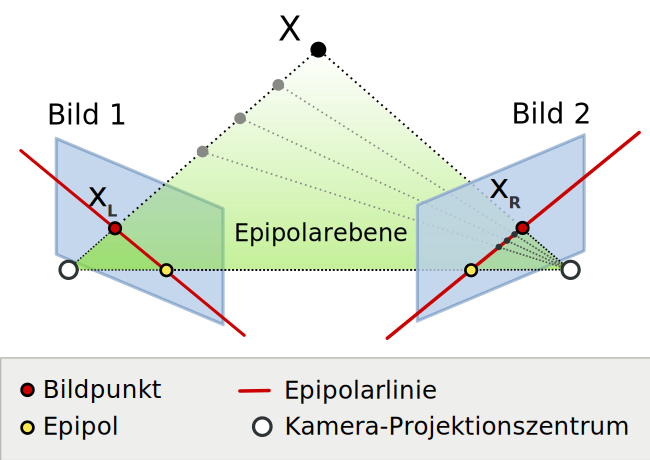
\includegraphics[width=217pt]{includes/Epipolargeometrie3}\\
		Quelle: http://de.wikipedia.org/wiki/Epipolargeometrie
	\end{center}
\end{frame}


\begin{frame}
	\frametitle{Shape from Motion}
	\framesubtitle{Orientierung berechnen}
	
	\begin{itemize}
		\item Lineares Gleichungssystem aufbauen und lösen.
		\item Relative Orientierungen von allen Kamerapaaren kombinieren.
	\end{itemize}
\end{frame}


\subsection{Erweiterungen}
\begin{frame}
	\frametitle{Shape from Motion}
	\framesubtitle{Erweiterungen}
	
	\begin{itemize}
		\item Bundle adjustment (Fehler minimieren)
		\item Dense Matching (Punktwolke verdichten)
		\item Oberfläche konstruieren
	\end{itemize}
\end{frame}

% ---------------------------------------------------------------------------- %

\section{Shape from Shading}
\subsection{MISSING}
\begin{frame}
	\frametitle{Shape from Shading}
	
	Missing content will be added soon.
\end{frame}

% ---------------------------------------------------------------------------- %

\section{Shape from Texture}
\frame{
	\frametitle{Shape from Texture}
	\framesubtitle{Einleitung}
	\begin{figure}
	\stackunder{\includegraphics[width=99px, height = 80px]{includes/sft_texture_2}}{Fig. 1}
	\stackunder{\includegraphics[width=105px, height = 80px]{includes/sft_texture_1}}{Fig. 2}
	\end{figure}

	\begin{itemize}
		\item Objekt mit texturierter Oberfläche rekonstruieren
		\item Textur besteht aus sich wiederholenden Texturelementen (Texel)
		\item Unterscheidung zwischen globalen und lokalen Verfahren
	\end{itemize}
}

\frame{
	\frametitle{Shape from Texture}
	\framesubtitle{Einleitung}
	\begin{figure}
	\stackunder{\includegraphics[width=230px, height = 120px]{includes/sft_slant-tilt}}{Fig. 3}
	\end{figure}
	\begin{itemize}
		\item slant $\rho$: Winkel zwischen $z_s$ und $z_i$\\
		\item tilt $\tau$: Winkel zwischen Projektion von $z_s$ auf Bildebene und $x_i$\\
		\item Normale: $z_s = \begin{pmatrix}
			\sin \rho \cos \tau\\
			\sin \rho \sin \tau\\
			\cos \rho
			\end{pmatrix}$
	\end{itemize}
	}

\frame{
	\frametitle{Shape from Texture}
	\framesubtitle{Ergebnis}
	
	\begin{figure}
	\stackunder{\includegraphics[width=300px, height = 96px]{includes/sft_result}}{Fig. 4}
	\stackunder{\includegraphics[width=300px, height = 81px]{includes/sft_result2}}{Fig. 5}
	\end{figure}
}

% ---------------------------------------------------------------------------- %

\section{Quellenverzeichnis}
\begin{frame}
	\frametitle{Quellenverzeichnis}
	\framesubtitle{Shape from Motion}
	
	\begin{tiny}
	\begin{itemize}
		\item \href{http://tu-dresden.de/die\_tu\_dresden/fakultaeten/fakultaet\_forst\_geo\_und\_hydrowissenschaften/fachrichtung\_geowissenschaften/ipf/photogrammetrie/elearning/software\_sfm}{http://tu-dresden.de/die\_tu\_dresden/fakultaeten/fakultaet\_forst\_geo\_und\_hydrowissenschaften/fachrichtung\_geowissenschaften/ipf/photogrammetrie/elearning/software\_sfm}
		\item \href{http://de.wikipedia.org/wiki/Bildregistrierung}{http://de.wikipedia.org/wiki/Bildregistrierung}
		\item \href{http://de.wikipedia.org/wiki/Epipolargeometrie}{http://de.wikipedia.org/wiki/Epipolargeometrie}
		\item \href{http://en.wikipedia.org/wiki/Scale-invariant_feature_transform}{http://en.wikipedia.org/wiki/Scale-invariant\_feature\_transform}
		\item \href{http://www.cs.cornell.edu/~snavely/bundler/}{http://www.cs.cornell.edu/$\sim$snavely/bundler/}
		\item \href{https://github.com/snavely/bundler_sfm/blob/master/RunBundler.sh}{https://github.com/snavely/bundler\_sfm/blob/master/RunBundler.sh}
		\item \href{http://www.di.ens.fr/pmvs/}{http://www.di.ens.fr/pmvs/}
		\item \href{http://www.igp.ethz.ch/photogrammetry/education/lehrveranstaltungen/PCV_HS12/content_folder/PCV-HS2012-slides-multiview.pdf}{http://www.igp.ethz.ch/photogrammetry/education/lehrveranstaltungen/PCV\_HS12/content\_folder/PCV-HS2012-slides-multiview.pdf}
		\item \href{http://mi.eng.cam.ac.uk/~cipolla/publications/contributionToEditedBook/2008-SFM-chapters.pdf}{http://mi.eng.cam.ac.uk/$\sim$cipolla/publications/contributionToEditedBook/2008-SFM-chapters.pdf}
	\end{itemize}
	\end{tiny}
\end{frame}


\begin{frame}
	\frametitle{Quellenverzeichnis}
	\framesubtitle{Shape from Texture}
	
	\begin{tiny}
	\begin{itemize}
	\item \href{http://homepages.inf.ed.ac.uk/rbf/CVonline/LOCAL_COPIES/AV0506/s0565925.pdf}{http://homepages.inf.ed.ac.uk/rbf/CVonline/LOCAL\_COPIES/AV0506/s0565925.pdf}
	\item \href{https://www.eecs.berkeley.edu/Research/Projects/CS/vision/papers/forsyth-iccv01.pdf}{ttps://www.eecs.berkeley.edu/Research/Projects/CS/vision/papers/forsyth-iccv01.pdf}
	\item \href{http://classes.soe.ucsc.edu/cmpe264/Spring04/Lec18.pdf}{http://classes.soe.ucsc.edu/cmpe264/Spring04/Lec18.pdf}
	\item \href{http://www.bmva.org/bmvc/2005/papers/34/paper.pdf}{http://www.bmva.org/bmvc/2005/papers/34/paper.pdf}
	\end{itemize}
	\begin{itemize}
	\item Fig.1: \href{http://upload.wikimedia.org/wikipedia/commons/2/2c/Acinonyx_jubatus_-Southern_Namibia-8.jpg}{http://upload.wikimedia.org/wikipedia/commons/2/2c/Acinonyx\_jubatus\_-Southern\_Namibia-8.jpg}
	\item Fig.2, Fig.4: \href{http://www.bmva.org/bmvc/2005/papers/34/paper.pdf}{http://www.bmva.org/bmvc/2005/papers/34/paper.pdf}
	\item Fig.3: \href{http://homepages.inf.ed.ac.uk/rbf/CVonline/LOCAL_COPIES/AV0506/s0565925.pdf}{http://homepages.inf.ed.ac.uk/rbf/CVonline/LOCAL\_COPIES/AV0506/s0565925.pdf}
	\item Fig.5: \href{https://www.eecs.berkeley.edu/Research/Projects/CS/vision/papers/forsyth-iccv01.pdf}{https://www.eecs.berkeley.edu/Research/Projects/CS/vision/papers/forsyth-iccv01.pdf}
	\end{itemize}
	\end{tiny}
\end{frame}


%http://tu-dresden.de/die_tu_dresden/fakultaeten/fakultaet_forst_geo_und_hydrowissenschaften/fachrichtung_geowissenschaften/ipf/photogrammetrie/elearning/software_sfm
%http://de.wikipedia.org/wiki/Bildregistrierung
%http://de.wikipedia.org/wiki/Epipolargeometrie
%http://en.wikipedia.org/wiki/Scale-invariant_feature_transform
%http://www.cs.cornell.edu/~snavely/bundler/
%https://github.com/snavely/bundler_sfm/blob/master/RunBundler.sh
%http://www.di.ens.fr/pmvs/
%http://www.igp.ethz.ch/photogrammetry/education/lehrveranstaltungen/PCV_HS12/content_folder/PCV-HS2012-slides-multiview.pdf
%http://mi.eng.cam.ac.uk/~cipolla/publications/contributionToEditedBook/2008-SFM-chapters.pdf

%http://www.cs.umd.edu/~mount/ANN/
%http://users.ics.forth.gr/~lourakis/sba/
%https://github.com/TheFrenchLeaf/Bundler/blob/master/src/keys2a.cpp
%https://github.com/TheFrenchLeaf/Bundler/blob/master/src/KeyMatchFull.cpp


\end{document}
